% testing.tex
\chapter{Testing}

\section{Test Strategy}
In this section I will compare my my finished project with the original specification proposed in my Analysis section. I will be conducting a series of tests to see if the app meets the original requirements. I will be testing the backend and frontend separately. 

Video demonstration of the app will be provided to show the app in action, this will provide a complete overview of the app and its features. This is my acceptance testing as it will show the app working and meets the original requirements.

The primary testing strategy for my backend project would be Unit testing to see if all the smaller components of my app work as intended. Django provide its own testing framework built on top of Python's unittest module. I will be using this to test my models and the methods within them, as well as the utility functions I have created in my app. Normal, boundary and edge cases will be tested where applicable. In addition, screenshots of the PostgreSQL database will also be shown.

For the API endpoints I will be using REST client provided by Visual Studio Code to make HTTP requests to the server and compare the result with my anticipated result. I will be doing this rather than using Django's own testing framework because I want to model real world usage of my app by making legitimate HTTP requests to actually modify the database.

For my frontend Interface, I will be will be testing the app manually by interacting with the components to see if the app behaves as expected. This is also act as my integration testing as I will be testing the app as a whole - frontend depends on the backend.

\subsection{Unit Testing}
\subsubsection{User}
Here are the unit tests I have written for the User model in my app:
\begin{minted}{python3}
    from django.test import TestCase
from django.core.exceptions import ValidationError
from Users.models import MyUser
from .utils import validate_email, clean_email, hash_password, verify_password

from django.test import TestCase
from .utils import hash_password, verify_password, validate_email, clean_email


class UtilityFunctionTests(TestCase):

    def test_hash_password(self):
        password = "testpassword123"
        hashed_password = hash_password(password)
        self.assertIsInstance(hashed_password, str)
        self.assertTrue(":" in hashed_password)

    def test_verify_password(self):
        password = "testpassword123"
        hashed_password = hash_password(password)
        self.assertTrue(verify_password(password, hashed_password))

    def test_verify_password_incorrect(self):
        password = "testpassword123"
        incorrect_password = "wrongpassword"
        hashed_password = hash_password(password)
        self.assertFalse(verify_password(incorrect_password, hashed_password))

    def test_validate_email_valid(self):
        valid_email = "test@test.com"
        self.assertTrue(validate_email(valid_email))

    def test_validate_email_invalid(self):
        invalid_email = "not-an-email"
        self.assertFalse(validate_email(invalid_email))

    def test_clean_email_valid(self):
        valid_email = "test@test.com"
        self.assertEqual(clean_email(valid_email), valid_email)

    def test_clean_email_all_caps(self):
        test_email = "TEST@TEST.COM"
        self.assertEqual(clean_email(test_email), test_email.lower())

    def test_clean_email_with_extra_characters(self):
        valid_email = "      test@test.com  "
        self.assertEqual(clean_email(valid_email), "test@test.com")


class MyUserModelTests(TestCase):

    def test_create_user(self):
        email = "test@test.com"
        password = "password"
        user: MyUser = MyUser.objects.create_user(email=email, password=password)
        self.assertEqual(user.email, email)
        self.assertTrue(user.check_password(password))

    def test_create_user_invalid_email(self):
        email = "not-an-email"
        password = "password"
        with self.assertRaises(ValueError):
            MyUser.objects.create_user(email=email, password=password)
\end{minted}

\begin{figure}[H]
    \centering
    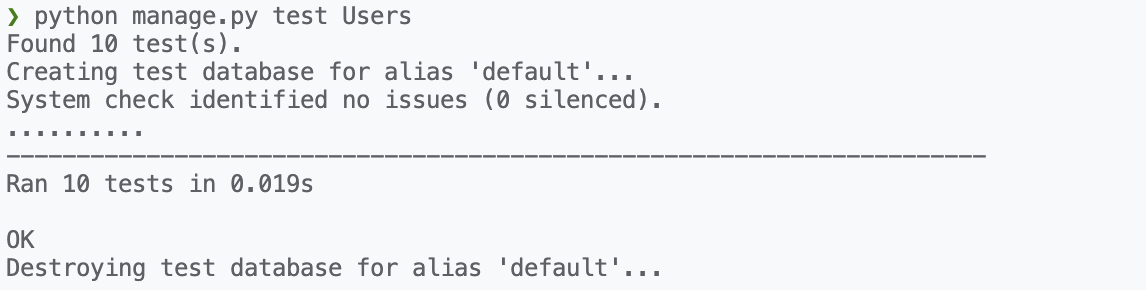
\includegraphics[width=\textwidth]{Assets/users_test_result.png}
    \caption{Unit Test Result for User App in Django}
    \label{fig:unit_test_user}
\end{figure}

\subsubsection{Journal}



\section{Endpoints}
To model real world usage, I will be making HTTP requests to the server and compare the result with my anticipated result. Here are a list of views created in my app:

\begin{minted}{python3}
    # from entries/urls.py
    urlpatterns = [
        re_path("sample/", views.sampleEntry, name="sample entry"),
        re_path("testUser/", views.test_user, name="test user"),
        re_path("getEntries/", views.get_all_entries, name="get all entries"),
        re_path("createEntry/", views.create_entry, name="create entry"),
        re_path(
            "getScheduledUsers/",
            views.get_daily_scheduled_email_users,
            name="get scheduled email users",
        ),
        re_path("deleteEntry/", views.delete_entry, name="delete entry"),
        re_path(
            "getJournalStatistics/",
            views.get_journal_statistics,
            name="get entry statistics",
        ),
    ]
\end{minted}


\begin{minted}{python3}
    # from users/urls.py
    urlpatterns = [
        re_path("register/", views.register_view, name="api_register"),
        re_path("login/", views.login_view, name="api_login"),
        re_path("logout/", views.logout_view, name="api_logout"),
        re_path("test_user/", views.test_user, name="test_user"),
        # re_path("update_email_prompt/", views.update_email_prompt, name="email_prompt"),
        # path("session/", views.session_view, name="api_session"),
    ]
\end{minted}

Here are the tests for relevant endpoint:
\subsection{sample/}
\subsection{testUser/}
\subsection{getEntries/}
\subsection{deleteEntry/}
\subsection{getJournalStatistics/}
\subsection{register/}
\subsection{login/}
\subsection{logout/}
\subsection{test\_user/}


\subsection{Rest Client}


\section{Frontend Interface}    
TODO: Frontend Interface

\section{Testing Video}
Include a link or description of a testing video.
TODO: Test video

\section{System Tests}
Conduct tests against the original requirements specification.
TODO: System tests



